\documentclass[12pt]{report}
\usepackage{amsmath, amssymb, amsthm, mathtools, geometry, graphicx, tikz, pgfplots, hyperref}
\usetikzlibrary{arrows.meta, angles, quotes, calc}
\usepackage{indentfirst}

\title{Elementary Complex Analysis}
\author{$\mathbb{Z}$heng Wai Hong}
\date{A.D. 2026.07.07}

\newtheoremstyle{mydefstyle}
    {1em}          % 上方间距（保持默认）
    {1em}          % 下方间距（保持默认）
    {\normalfont}  % 正文字体（常规，不加粗）
    {0pt}          % 首行缩进（0 表示无额外缩进）
    {\bfseries}    % 标题字体（加粗！）
    { }            % 标题后的标点符号（这里改为句点，也可以不要）
    { }            % 标点后的空格
    {\thmname{#1} \thmnumber{#2}: \thmnote{#3}\newline}  % 关键：末尾加了 \newline，实现换行
% 应用该样式
\theoremstyle{mydefstyle}

\newcommand{\RR}{\mathbb{R}}
\newcommand{\CC}{\mathbb{C}}
\newcommand{\ZZ}{\mathbb{Z}}
\newcommand{\QQ}{\mathbb{Q}}
\newcommand{\NN}{\mathbb{N}}
\newcommand{\RE}{\mathrm{Re}}
\newcommand{\IM}{\mathrm{Im}}
\newcommand{\Par}{\partial}

\begin{document}

\newtheorem{theorem}{Theorem}[section]
\newtheorem{lemma}[theorem]{Lemma}
\newtheorem{corollary}[theorem]{Corollary}
\newtheorem{proposition}[theorem]{Proposition}
\newtheorem{definition}{Definition}[section]

\maketitle
\begin{abstract}
    This is a text of elementary complex analysis referencing "COMPLEX ANALYSIS" of Elias Stein and Rami Shakarchi.
    \begin{figure}[htbp]
        \centering
        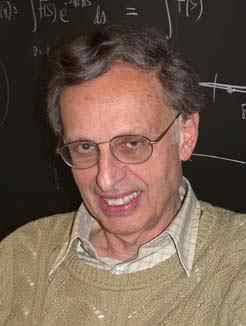
\includegraphics[width=0.5\textwidth]{../../photos/Elias_Stein.jpg}
        \caption{Elias Stein}
    \end{figure}
\end{abstract}

\tableofcontents

\newpage

\chapter{Complex Numbers and Complex Functions}

\section{Complex Numbers}

Before systematically learning complex analysis, we have to first understand the complex numbers $\CC$ . One might have heard that the complex numbers were introduced to solve the problems of the non-real roots of polynomial equations. For instance that considering the equation
\[ 0=x^2+1 \]
In reals, it is impossible for certain $x_0 \in \RR$ such that its square is negative. Thus, we introduce the imaginary unit $i$ defined by
\[ i^2=-1 \]
and we endow the scalar multiplication for $yi$ where $y \in \RR$ . Then, we define the complex numbers by the forms of $z=x+yi$ where $x,y \in \RR$ and called the real Part and the imaginary Part of $z$ respectively, denoted by $\RE(z)$ and $\IM(z)$ . 

The operations of complex numbers are defined by the respective operations of the real Part and the imaginary Part. If $z=x+yi$ and $w=a+bi$ , then
\[ z+w=(\RE(z)+\RE(w))+(\IM(z)+\IM(w))i=(x+a)+(y+b)i \]
\[ z \ w = (x+yi)(a+bi)= (xa-yb)+(xb+ya)i \]
\[ \frac{z}{w}=\frac{x+yi}{a+bi}=\left(\frac{x+yi}{a+bi}\right)\left(\frac{a-bi}{a-bi}\right)=\frac{1}{a^2+b^2}\left( (xa+yb)+(ya-xb)i \right) \]
Based on the operations above, we can easily deduce the algebraic properties of $\CC$ , for $z_1,z_2,z_3 \in \CC$ :
\begin{itemize}
    \item Commutativity: $z_1+z_2=z_2+z_1, z_1z_2=z_2z_1$
    \item Associativity: $(z_1+z_2)+z_3=z_1+(z_2+z_3), (z_1z_2)z_3=z_1(z_2z_3)$
    \item Distributivity: $z_1(z_2+z_3)=z_1z_2+z_1z_3$
\end{itemize}

Note that we can use an ordered pair $(x,y)\in \RR^2$ to uniquely determinea a complex number $x+yi$ so that in terms of topology, $\CC$ is homeomorphic to $\RR^2$ and we can use a plane to represent $\CC$ , called complex plane. Therefore, we can directly apply the topology of $\RR^2$ to $\CC$ , such as convergence, connectedness, compactness, and etc.

\begin{figure}[htbp]
    \centering
    \begin{tikzpicture}[scale=1.0]
        % 定义复数的实部和虚部
        \def\a{2.5}   % 实部 x
        \def\b{1.8}   % 虚部 x

        % ---------- 坐标轴 ----------
        \draw[->, thick] (-3,0) -- (4,0) node[right] {Re};
        \draw[->, thick] (0,-2) -- (0,3) node[above] {Im};
        \node[below left] at (0,0) {$0$};

        % ---------- 绘制向量（从原点到 a+bi） ----------
        \draw[->, thick, black] (0,0) -- (\a,\b) node[midway, above right]{};

        % ---------- 标记点 ----------
        \filldraw (\a,\b) circle (1.0pt) node[above right] {$x+yi$};

        % ---------- 投影虚线（从点到实轴、虚轴） ----------
        \draw[dashed, gray] (\a,0) -- (\a,\b) -- (0,\b);

        % ---------- 在实轴和虚轴上标记 a 和 b ----------
        \node[below] at (\a,0) {$a$};
        \node[left] at (0,\b) {$bi$};

        % ---------- 绘制辐角弧（从实轴到向量） ----------
        \coordinate (O) at (0,0);
        \coordinate (A) at (\a,0);
        \coordinate (B) at (\a,\b);
        \pic[draw, black, ->, angle radius=0.5cm, angle eccentricity=1.3] {angle = A--O--B};
        \node at (0.7,-0.3) {$\arg(z)$};
    \end{tikzpicture}
    \caption{Complex Plane}
\end{figure}

Next, we introduce some important terms of complex numbers. The magnitude of a complex number $z=x+yi$, denoted by $|z|$ , is defined by
\[ |z|=\sqrt{x^2+y^2} \]
The argument of $z$ , denoted by $\arg(z)$ is defined by the angle between $z$ and the real axis
\[ \arg(z)=\arctan\frac{y}{x} \]
The conjugate of $z$ , denoted by $\bar{z}$ , is a complex number such that 
\[ \bar{z}=x-yi \]
which is exactly the complex number with the opposite imaginary Part of $z$ . Clearly, if $z \in \RR$ , $\bar{z}=z$ and if $z = yi$ , $\bar{z}=-z$ . And, one should notice that $|z|^2=z \bar{z}$ . 

A useful and prominent result found by Euler is the polar form of the complex numbers, that since 
\[ \sin \theta = \frac{e^{i \theta}-e^{-i\theta}}{2i}, \cos \theta = \frac{e^{i \theta}+e^{-i\theta}}{2} \]
and 
\[ z=x+yi=|z|\left(\frac{x}{|z|}+\frac{y}{|z|}i\right)=|z|(\cos \theta + i \sin \theta) \]
we have 
\[ z= |z| e^{i\theta} \]
where $\theta = \arg(z)$ . If $z$ is unit, then 
\[ e^{i x} = \cos x + i \sin x \]
which is called the Euler Formula, playing a pivotal role in Math.

Let $z=r e^{i \varphi}$ and $w = s e^{i \theta}$ , then
\[ zw = rs \ e^{i (\varphi + \theta)} \]
so that the multiplication of the complex numbers actualy conducts a rotation in the plane.

\section{Complex Functions}
It is no surprise for those who have learned the multivariable functions when first encountering the complex functions.  The formal form ofthe  complex functions are the maps $f:\CC \longrightarrow \CC, z \mapsto f(z)$ . Since the complex numbers have actually two variables, which are the real and the imaginary Part, the complex functions are essentially a type of two-variable functions. However, the definition that $i^2=-1$ make them be distinct from the general two-variable functions.

We first introduce the continuous functions, which is defined as usual.

\begin{definition}[Continuous functions]
\label{def:Continuous functions}
    Let $f$ be a function defined on a set $\Omega \subset \CC$ . Then, $f$ is continuous at $z_0 \in \Omega$ if $\forall \varepsilon>0, \exists \delta>0$ such that $\forall z \in \Omega$ , 
    \[ |z-z_0|<\delta \implies |f(z)-f(z_0)|<\varepsilon \]
    $f$ is continuous on $\Omega$ if $f$ is continuous at all $z \in \Omega$ .
\end{definition}

Since $\CC \cong \RR^2$ , we can also express the definition above by the form of balls.
\[ \forall \varepsilon>0, \exists \delta>0, \forall z \in \Omega, z \in B_{\delta}(z_0) \implies f(z) \in B_{\varepsilon}(f(z_0)) \]

Moreover, an equivalent definition of continuity is by the limit of sequence that if $f$ is continuous at $z_0$ , then 
\[ \forall \{z_n\}_{n=1}^{\infty} \subset \Omega, \lim_{n \to \infty}z_n = z_0 \implies \lim_{n \to \infty}f(z_n) = f(z_0) \]
\begin{figure}[htbp]
\centering
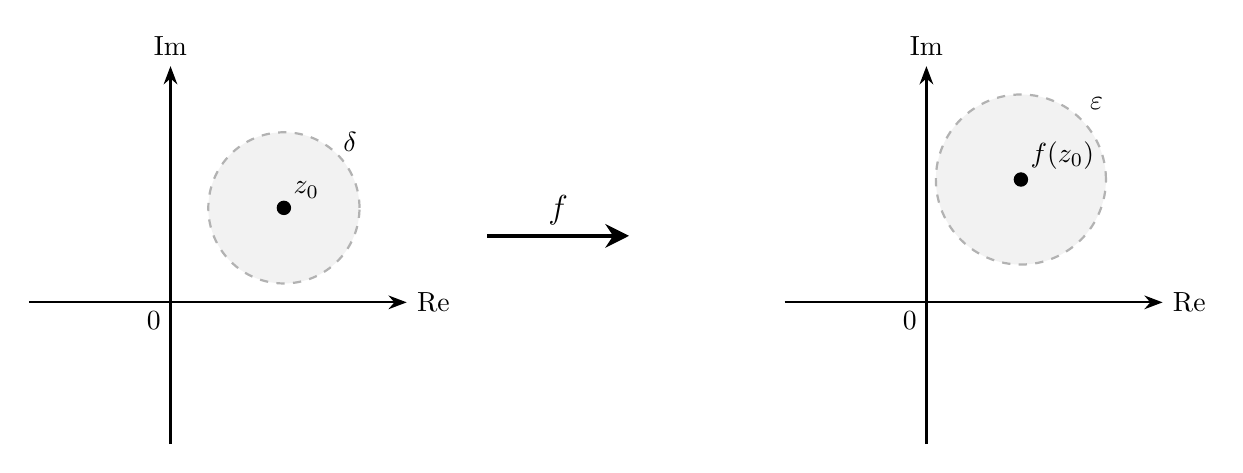
\begin{tikzpicture}[scale=1.2, >=Stealth]

% ===== 左侧 z-平面 =====
\begin{scope}[xshift=-4cm, local bounding box=zplane]
    \draw[->, thick] (-1.5,0) -- (2.5,0) node[right] {Re};
    \draw[->, thick] (0,-1.5) -- (0,2.5) node[above] {Im};
    \node[below left] at (0,0) {$0$};

    \def\zx{1.2}
    \def\zy{1.0}
    \def\radiusDelta{0.8}   % 改用新名字存储半径数值

    % 圆盘（δ-邻域）
    \draw[black!30, fill=gray!10, dashed, thick] (\zx,\zy) circle (\radiusDelta);  % 使用新名字
    \node at (\zx+0.7, \zy+0.7) {$\delta$};   % 这里仍然是希腊字母符号

    % 点 z0
    \filldraw (\zx,\zy) circle (2pt) node[above right] {$z_0$};
\end{scope}

% ===== 中间箭头 =====
\draw[->, very thick, -{Stealth[length=3mm, width=3mm]}] 
    ($(zplane.east)+(0.3,0)$) -- ($(zplane.east)+(1.8,0)$)
    node[midway, above, font=\large] {$f$};

% ===== 右侧 w-平面 =====
\begin{scope}[xshift=4cm, local bounding box=wplane]
    \draw[->, thick] (-1.5,0) -- (2.5,0) node[right] {Re};
    \draw[->, thick] (0,-1.5) -- (0,2.5) node[above] {Im};
    \node[below left] at (0,0) {$0$};

    \def\wx{1.0}
    \def\wy{1.3}
    \def\radiusEpsilon{0.9}   % 改用新名字

    \draw[black!30, fill=gray!10, dashed, thick] (\wx,\wy) circle (\radiusEpsilon);
    \node at (\wx+0.8, \wy+0.8) {$\varepsilon$};   % 仍然是希腊字母

    \filldraw (\wx,\wy) circle (2pt) node[above right] {$f(z_0)$};
\end{scope}

\end{tikzpicture}
\caption{Visualisation of continuous complex functions}
\label{fig:mapping}
\end{figure}

For real continuous functions, we have known that they always attain the extreme in a compact set. We can define the similar concept by the magnitude of the functions that $f$ attains a maximum at $z_0 \in \Omega$ if 
\[ \forall z \in \Omega, |f(z)| \leqslant |f(z_0)| \]
with the inequality reversed for the definition of a minimum. 

Note that by the triangle inequality, $|f|$ is continuous if $f$ is continuous. Indeed
\[ \left|\ |f(z_0)|-|f(z)|\ \right|\leqslant |f(z_0)-f(z)| \]
We can deduce a plenty of properties of the magnitude of the complex functions according to the continuity of $|f(z)|$ .

\begin{theorem}
\label{the:extreme of continuous functions}
    A continuous functions on a compact set $\Omega$ is bounded and attains a maximum and minimum on $\Omega$ .
\end{theorem}

\begin{theorem}
\label{the:mean value property}
    Let $f$ be a continuous function on $\Omega \subset \CC$ , and denote by $M=\max_{z \in \Omega}|f(z)|$ , $m=\min_{z \in \Omega}|f(z)|$ . Then, 
    \[ \forall y \in [m,M] , \exists z_0 \in \Omega: |f(z_0)|=y \]
\end{theorem}

The theorems here follow immediately from the properties of single-variable continuous functions.

\section{Holomorphic Functions}

Now, we discuss the derivative of complex functions.

\begin{definition}[Holomorphic Functions]
\label{def:holomorphi functions}
    Let $\Omega$ be an open set in $\CC$ and $f$ a complex-valued function on $\Omega$ . Then, $f$ is holomorphic at $z_0 \in \Omega$ if the limit
    \[ \lim_{h\to 0}\frac{f(z_0+h)-f(z_0)}{h} \]
    converges where $h \in \CC$ and $z_0+h \in \Omega$ , and the limit is called the derivative of $f(z)$ at $z_0$ , denoted by $f'(z_0)$ . $f$ is holomorphic on $\Omega$ if $f$ is holomorphic at every point of $\Omega$ .
\end{definition}

The terms "complex differentiable" or "regular" are same to holomorphic. 

\begin{definition}[Entire Functions]
\label{def:entire functions}  
    If $f(z)$ is holomorphic at all $z \in \CC$ , then $f(z)$ is an entire function.
\end{definition}

In the following sections, you will see the advantages of holomorphic functions than differentiable function of single real variable. For example, the holomorphic functions are actually infinitely many times complex differentiable; the holomorphic functions can always be expanded to a power series so that we usually use the term "analytic" as a synonym for holomorphic.

A basic property of the holomorphic functions is its closure under the elementary operations.

\begin{proposition}
    If $f$ and $g$ are holomorphic in $\Omega$ , then
    \begin{itemize}
        \item $f+g$ is holomorphic in $\Omega$ and $(f+g)'=f'+g'$ .
        \item $f\ g$ is holomorphic in $\Omega$ and $f\ g = f'g+g'f$ .
        \item If $g(z_0) \neq 0$ , then $\frac{f}{g}$ is holomorphic at $z_0$ and
        \[ \left(\frac{f}{g}\right)'= \frac{f'g-fg'}{g^2} \]
        \item If $f: \Omega \longrightarrow U$ and $g:U \longrightarrow \CC$ are holomorphic, then the chain rule holds and
        \[ \forall z \in \Omega, \;(g\circ f)'=g'(f(z))f'(z) \]
    \end{itemize}
\end{proposition}

As the complex numbers are consisted of the ordered pair $(x,y)\in \RR^2$ , we can also write the complex functions with following form by $z=x+yi$
\[ f(x,y) = u(x,y)+v(x,y)i \]
where $u(x,y)= \RE(f(z)), v(x,y)=\IM(f(z))$ . Then, we can take the partial derivatives of $f$ as a multi-variable function
\[ \frac{\Par f}{\Par x} = \frac{\Par u(x,y)}{\Par x} + i \frac{\Par v(x,y)}{\Par x} \]
\[ \frac{\Par f}{\Par y} = \frac{\Par u(x,y)}{\Par y} + i \frac{\Par v(x,y)}{\Par y} \]

\end{document}